\chapter{Floatable Blocks}\label{ch:floats}

\marginpar{The research in\\ this chapter was previously published in \cite{Pinkney2013}}

% Required implementation:
% \begin{itemize}
%     \item extension of chapter 2 code to support floats
%     \item tradeoffs between Plass\cite{Plass1981} pagination and `dumb' pagination. Should floats be
%     `floatable'?
%     \begin{itemize}
%         \item how floatable?
%         \item how much effort do we put in before it stops being worth it?
%     \end{itemize}
%     \item Floats across multiple columns?
%     \begin{itemize}
%         \item simple multiples of galley width/line height
%     \end{itemize}
%     \item Bringhurst's suggestion\cite{Bringhurst2008} of making blocks take up multiples of the
%     leading to always keep text in phase (could even factor this into chapter 2 implementation)
% 
% \end{itemize}

\summary{
The system described in Chapter~\ref{ch:malleable} supports only simple documents that are composed solely from text. Most documents contain figures, diagrams, illustrations, or tables, and so we must give consideration towards how these should be handled.

In this chapter, we extend the work of the previous chapter to allow floatable graphical blocks, whose absolute position within a document's text may vary depending upon the layout.

Furthermore, we reimplement the system described in the previous chapter, moving away from \pdf{} and Adobe Acrobat, towards a new system based in \html{}, \css{} and JavaScript that is much more portable and as such can be used on ebook hardware.
}

%\section{Implementation}

The implementation of the system described in the previous chapter is deeply rooted within \gls{pdf}, and requires a custom-written plugin for Adobe Acrobat (see Section~\ref{sec:acroplugin}) to view the documents. Consequently, it is difficult to test that particular implementation on any device that is not running Microsoft Windows and does not have a fully licensed version of Adobe Acrobat, which effectively rules out any mobile \ebook{} readers.
Almost all \ebook{} readers support the \epub{} format,\marginpar{Amazon's \emph{Kindle} is one of the few contemporary devices that do not support \epub{}} which is principally built upon \html{}, \css{}, and JavaScript. With this in mind, it was decided that the system should be  reimplemented using these technologies, in order that it could be deployed on \ebook{} hardware. 



\section{Document Generation}
\label{sec:docgen}

%In the system described in the previous chapter, the generation of malleable documents was a rather labour-intensive process, involving the processing of the source document through \ditroff{} and \pdfdit{}. In the case of documents with galleys of more than one width, modifications needed to be made, by hand, to the Galley Structure Tree of the resultant \gls{pdf} files.

%Adding or removing characters to the source of a \gls{pdf} file is no trivial matter, since the \textsc{xref} table, which stores the byte offset of every \gls{COSObject} within a \gls{pdf} file, is no longer valid. (Acrobat does kindly offer to fix this problem if it detects it, but it has the side effect of discarding any \gls{pdf} data that it does not recognise, presumably in the name of optimisation. Clearly losing the Galley Structure Tree is undesirable.) The \textsc{xref} table can either be fixed programatically, or by a painstaking process involving a hex editor and a lot of patience. 

Since the new system no longer relies on \gls{cog}-\gls{pdf}, the reliance on \troff{} and \pdfdit{} is no longer present. Consequently, a sensible approach is to produce a completely bespoke typesetting tool, allowing unneeded features to be removed, together with the provision of some finer-grained control over other aspects. For example, it is important for this system that the the line-breaking and hyphenation algorithms can easily be changed.

In the new system, the source document is described in terms of separate logical blocks: a block is either designated as a `float', or as a `paragraph'. (Listing~\ref{lst:sourcedoc} contains an excerpt from a sample source document.) Floats are currently limited to referencing images only (with an optional size parameter). Paragraphs, on the other hand, are described by their desired textual content. This is deliberately simple. It is envisaged that in a real system, the source document would have a richer language, perhaps using Markdown, \xml{}, or a form similar to \LaTeX{} source.

\begin{lstlisting}[label=lst:sourcedoc,captionpos=b,float,basicstyle=\ttfamily\footnotesize,caption={[An excerpt from a sample source document]An excerpt from a sample source document, itself an excerpt from \cite{Pinkney2011}. The document is parsed from top to bottom. Paragraphs are separated by blank lines. Floats are specified by lines that begin \texttt{\_\_FLOAT} and contain a reference to an image. Subsequent lines, until the next \texttt{\_\_FLOAT} or \texttt{\_\_PARA} marker, are interpreted as the float caption.}]
3.1.3 pdfdit

Having generated the source document, it was processed with
ditroff to generate the intermediate code used to feed each
typesetter post-processor. This output is very expressive, and,
unlike TEX's DVI, contains enough information that post-
processors are easily able to locate the start and end of lines
and paragraphs within the document. This meant that only minimal
changes were needed to be made to the pdfdit package described in
[1] to implement our design.

__FLOAT fig4.png

Figure 4: Sample renderings from the Acrobat plugin at page
widths of 42, 48, and 54 em.

__PARA

The first change necessary was to decrease the granularity of the
output COGs, producing them at the line level, rather than at the
paragraph level. Secondly, some method of generating the
requisite tree representing the document structure was required.
This was solved by simply using the point at which the original
version of pdfdit would have started a new paragraph-level COG,
and, instead, starting a new paragraph-level block entry in the
document structure tree. Each subsequent line-level COG produced
can then be added as a child of this block.

Once the entire output file has been parsed, the tree
representations of the various width galleys are amalgamated
per-paragraph, as indicated in figure 3, and finally the PDF file
is serialised, replete with COGs and content tree.

\end{lstlisting}


Next, the source document is passed through a program termed the \emph{Paragraph Splitter} to produce the output that becomes the malleable document itself.

The Paragraph Splitter passes the text of each paragraph through an implementation of a line-breaking algorithm. The Knuth-Plass algorithm\hspace{0pt}\cite{Knuth1981} was used by the Paragaph Splitter instance that produced the layouts shown in Appendix~\ref{app:layouts}, though it is trivial to replace this with any other line-breaking algorithm.

Each paragraph is rendered multiple times, once for each \gls{galley} width, in order to produce the document's multiple \gls{galley} renderings. Each line of each rendering of every paragraph is converted into a list of its composite words. All of these words have an associated position offset value (as shown in Listing~\ref{lst:datajs}) which is later used when drawing the text, to ensure that each word is positioned on the line with the correct spacing. The general algorithm used is given in Listing~\ref{lst:parsplitter}.


\begin{lstlisting}[label=lst:parsplitter,language=c,captionpos=b,float,basicstyle=\ttfamily\footnotesize,caption={[Algorithm used by the Paragraph Splitter]The algorithm followed by the Paragraph Splitter. Firstly the source of the document is parsed to break it into its initial logical blocks: one block per paragraph and one block per float, in the order encountered in the document source. These blocks are then processed further depending on their type. Floats may be probed for their pixel dimensions if no size was specified, and are then added to the Galley Structure Tree. Paragraphs have their content passed through a line breaking algorithm, once for each specified width.}]
galleyStrucTree renderDocument(documentContent, galleyWidths[]) {
    parasAndFloats[] = parseDocumentSource(documentContent);
    galleyStrucTree = empty tree;
    foreach (item in parasAndFloats) {
        if (item is a floatable object) {
            if (dimensions are not specified) {
                read pixel dimensions from file;
            }
            add floatable object to galleyStrucTree;
        } else { /* therefore item is a paragraph */
            create empty paragraph container;
            foreach (width in galleyWidths) {
                pass item text through linebreaker using width;
                create empty galley container;
                foreach (line returned by linebreaker) {
                    add words and positioning data of line to galley container;
                }
                add galley container to paragraph container;
            }
            add paragraph container to galleyStrucTree;
        }
    }
    return galleyStrucTree;
}

parasAndFloats[] parseDocumentSource(documentContent) {
    step through documentContent line by line, returning the documentContent broken into an array of strings with one element per paragraph and per floatable object;
}

\end{lstlisting}


The content of the floats is largely left unchanged. A reference to the image, along with its required dimensions, is simply passed through to the output. If dimensions were not explicitly specified in the source document, the pixel size of the image itself is used, at 96~\textsc{dpi} (\ie{} 16 pixels becomes 12 \glspl{point}).

Finally, once the whole of the source document has been processed, the rendered content is output\ed in the form of the Galley Structure Tree shown in figure~\ref{fig:tree} on page \pageref{fig:tree}\ed encoded as a \gls{json} string. This becomes the data representing the source document, which, in conjunction with the viewer defined in the next section, becomes a \emph{malleable document}. A sample of this data is shown in Listing~\ref{lst:datajs}.

\begin{lstlisting}[label=lst:datajs,captionpos=b,float,language=c,stringstyle=\color{blue},basicstyle=\ttfamily\scriptsize,caption={[Excerpt from JavaScript data file]Excerpt from JavaScript data file representing a 3-galley document. Note that the title "Abstract" is treated as any normal paragraph and, as for any paragraph, is typeset once for each galley rendering (despite there being no difference between each rendering in this case). The first rendering of the first paragraph of the abstract begins below. For brevity's sake, subsequent renderings are not shown, but since the following galleys are typeset with a different \gls{measure}, the spacing and words per line will differ. At the top is an object representing a float, which contains values for \textcolor{red}width, \textcolor{red}height, and \textcolor{red}data.}]
[
  {
    "w": 952.5,
    "h": 342.75,
    "d": "<img style=\"width:100%\" src=\"fig0.png\" alt=\"Reflowable Documents Composed from\nPre-rendered Atomic Components\nAlexander J. Pinkney\nSteven R. Bagley\nDavid F. Brailsford\nDocument Engineering Lab.\nSchool of Computer Science\nUniversity of Nottingham\nNottingham, NG8 1BB, UK\n{azp|srb|dfb}@cs.nott.ac.uk\n\">"
  },
  [
    [
      [
        [0, "Abstract"]
      ]
    ],
    [
      [
        [0, "Abstract"]
      ]
    ],
    [
      [
        [0, "Abstract"]
      ]
    ]
  ],
  [
    [
      [
        [0, "Mobile"], [38.346, "eBook"], [73.356, "readers"]
      ],
      [
        [0, "are"], [17.334, "now"], [40.68, "commonplace"]
      ],
      [
        [0, "in"], [13.004, "today&#39;s"], [52, "society,"], [92.664, "but"]
      ],
      [
        [0, "their"], [26.334, "document"], [78, "layout"]
      ],
      [
        [0, "algorithms"], [53.736,"remain"], [89.46,"basic,"]
      ],
      [
        [0, "largely"],[35.724, "due"],[55.452, "to"],[67.188, "constraints"]
      ],
  /* truncated */

\end{lstlisting}


\section{The Viewer}
\label{sec:viewer}

In order to circumvent the web browser's default text-layout algorithm, and to ensure that the ``high quality'' pre-computed text layout is used, the absolute position of every word on each line must be specified, in a manner not dissimilar to the internals of a PDF file. The Paragraph Splitter described in the previous section ensures that all the information needed to lay out the text is contained within the generated \gls{json} string representing the Galley Structure Tree.


When the viewer is launched, it decides which is the most appropriate \gls{galley} rendering to display, based on a metric of which rendering will be most aesthetically pleasing. Since it works well, the metric defined in Chapter~\ref{ch:malleable} is used, which balances a penalty for excessive inter-column whitespace against a penalty for too many columns.

Although every \gls{galley} is rendered in the same \gls{point} size, this can be scaled up or down at view-time based on the preference of the user, to simulate \gls{point}-size changes. All dimensions other than the page size, such as the gaps between words, are scaled proportionally, to allow the text to remain correctly justified.




\subsection{Floats with a Queue}
\label{sec:floatqueue}
The first approach taken towards supporting floats took inspiration from \TeX, which places floats into a queue until it finds somewhere it deems appropriate to place the first float \cite{Plass1981, Knuth1984}. In order to emulate this, two queues were defined: the \emph{float queue}, and the \emph{line queue}.


If both queues are empty, as they will be at the start of the layout process, the Galley Structure Tree is traversed, and when the first paragraph-level item (see Figure~\ref{fig:tree} on page~\pageref{fig:tree}) is encountered, its subcomponents (of the chosen \gls{galley} rendering) are added to the requisite queue: lines to the line queue, and floats to the float queue.

When at least one of the queues is not empty, document layout begins. If the float queue is non-empty, and the first float in the queue will fit below the last typeset item, it is placed on the page. If not, items from the line queue are placed one by one, until no more will fit in the current column. When this happens, a new column is started, and the first float in the float queue is output. Whenever the line queue is depleted, and no floats in the float queue will fit at the current point on the page, all subcomponents of the next paragraph-level item from the Galley Structure Tree are queued. This process is illustrated in Figure~\ref{fig:float-flowchart}.

\begin{figure}
  \begin{center}
  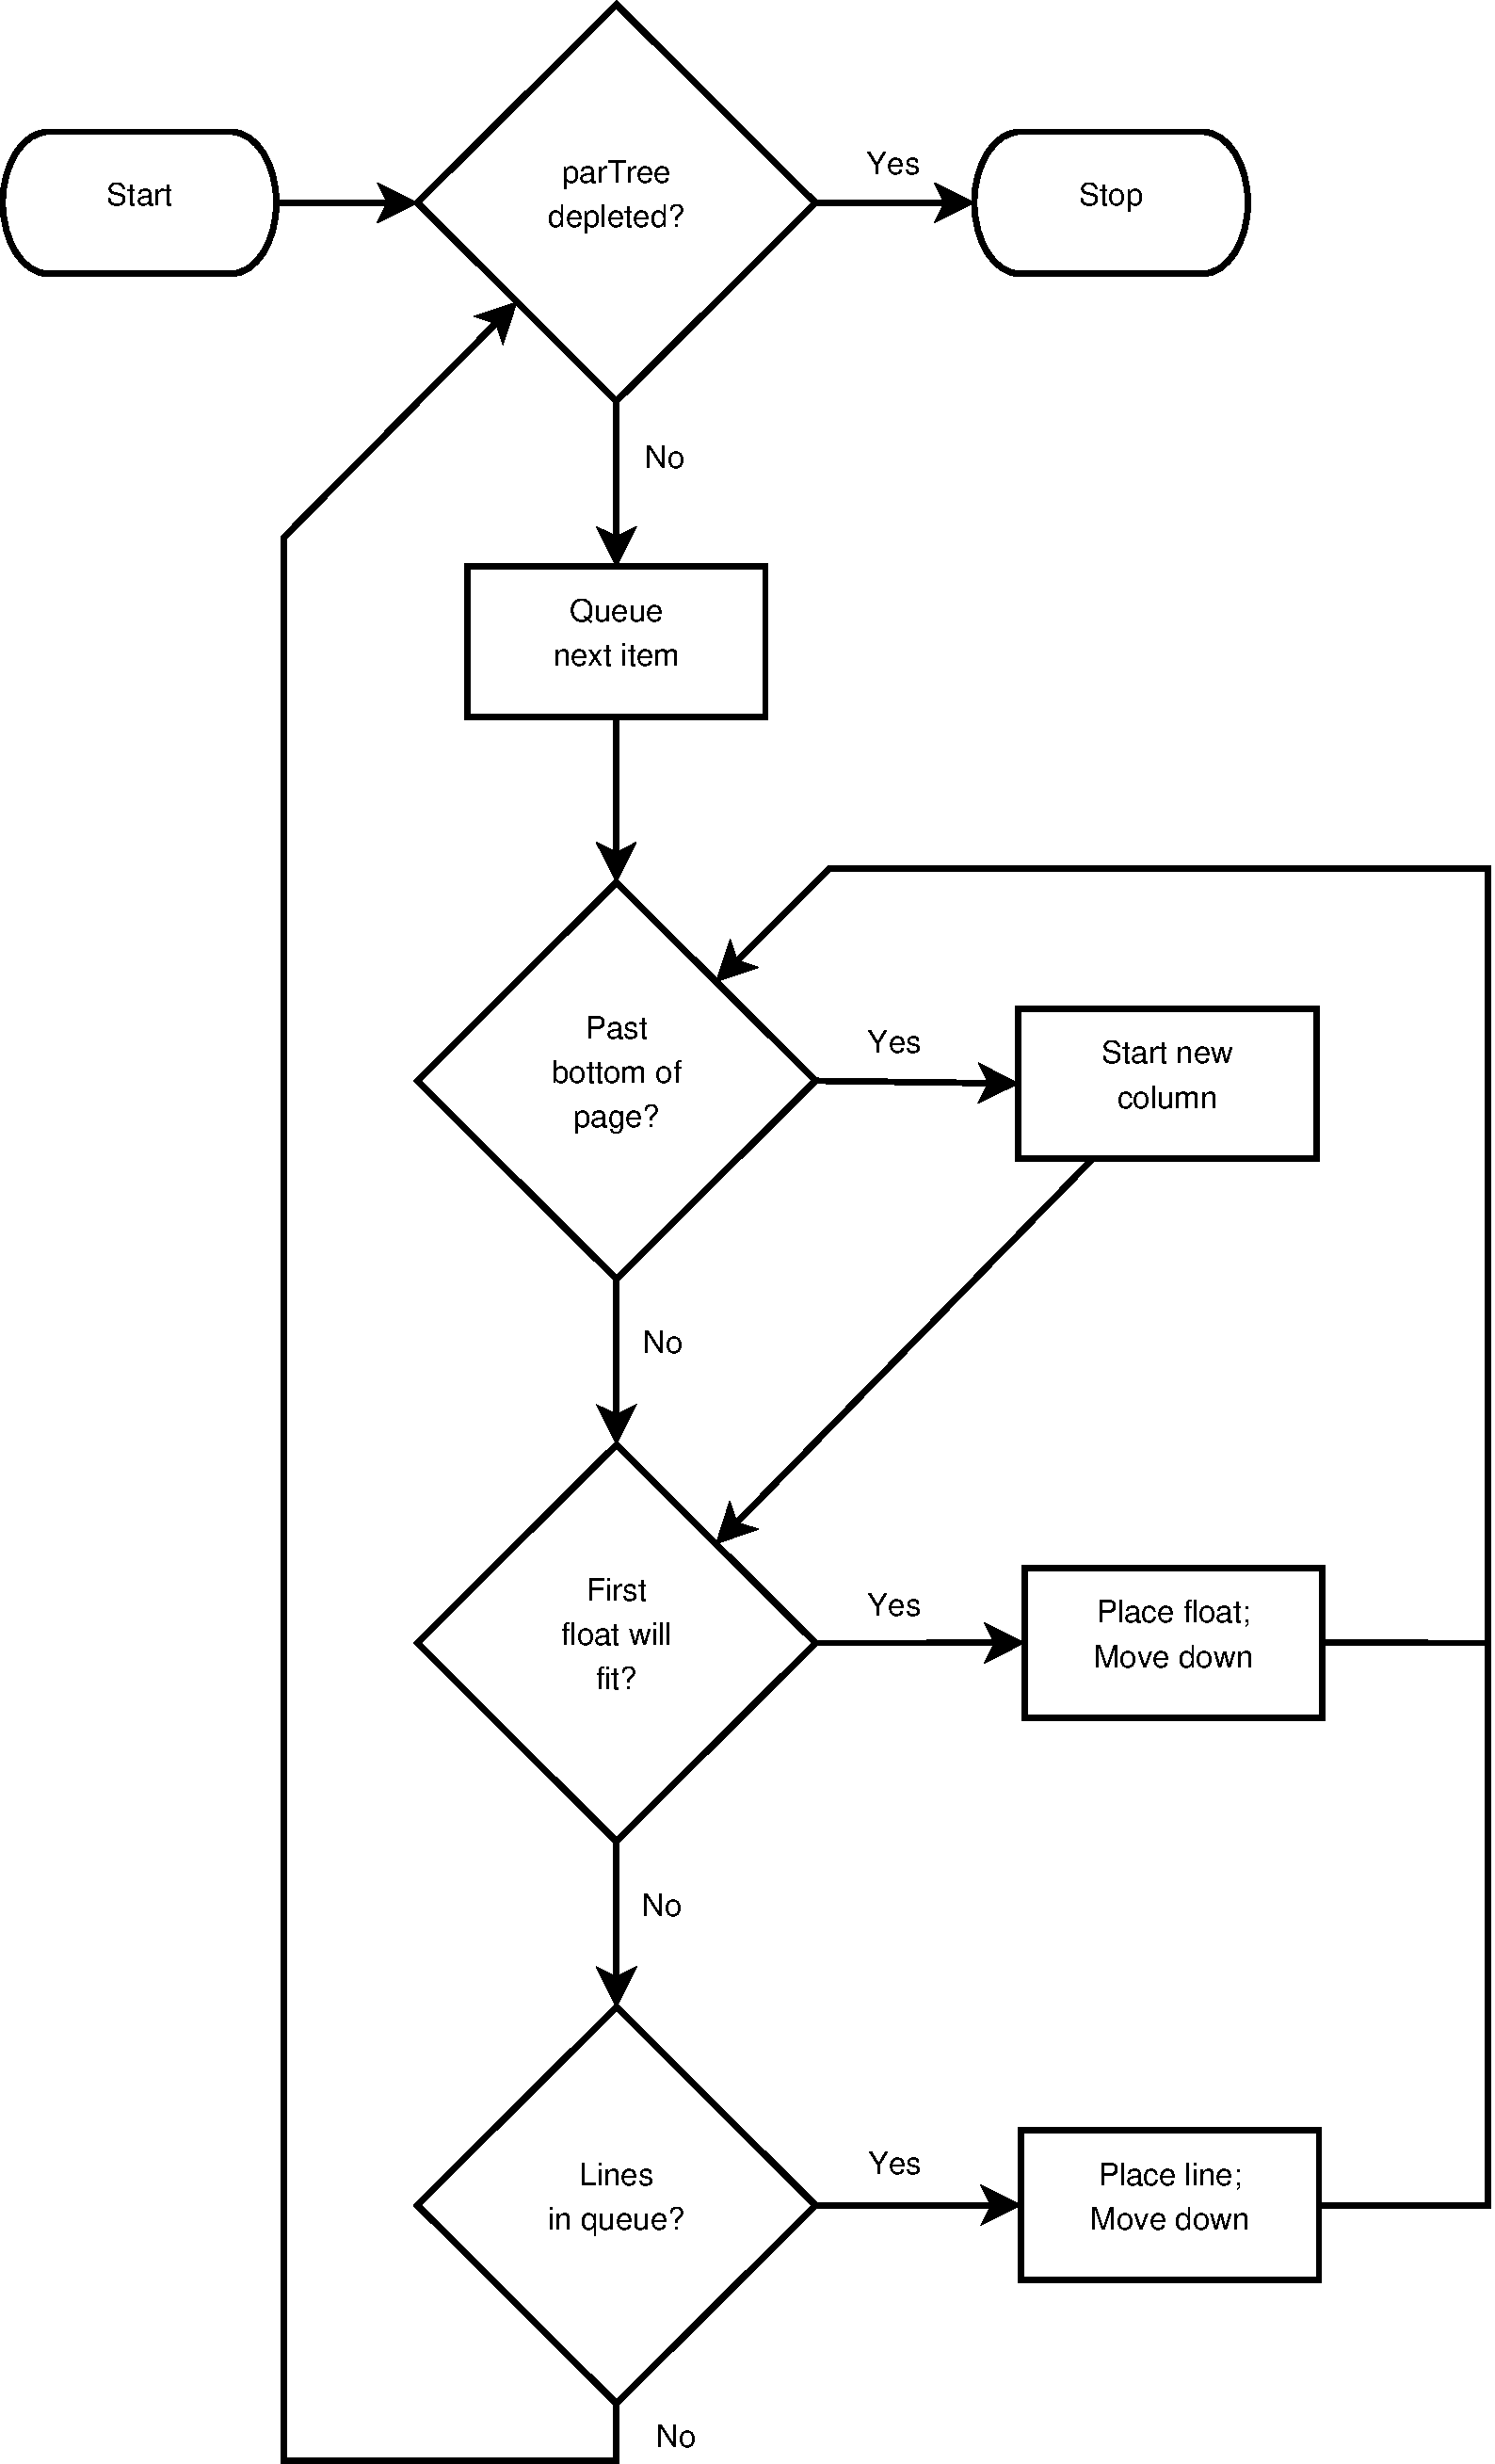
\includegraphics[width=\textwidth]{gfx/flowchart}
  \end{center}
  \caption[Flowchart of the two-queue float algorithm]{Flowchart describing the two-queue float algorithm. Section~\ref{sec:floatqueue} explains this process in detail.}
  \label{fig:float-flowchart}
\end{figure}

Pagination is reasonably simple with this queueing system: as soon as a page is full, the layout can be restarted at the origin of the page using the current status of both queues and the Galley Structure Tree. Whilst this approach does produce professional-looking layouts, and handles floats well without the need for backtracking, it is not particularly conducive to producing layouts with floats that span multiple columns. The queue-based layout described above is rather simplistic: it knows about the size of each component that it lays out, but it does not remember the history of the positions of any of the components that are already laid out. This makes it difficult to have items that span more than one column, because there is no mechanism to mark space on the page as being reserved. In order to do this, another approach must be taken.

\subsection{A Grid-Based Layout}
\label{sec:gridlayout}
% - Support of floats
    % - Queue system
    % - Grid/array system (no need for queue)
    % - Multicolumn floats
        % - issues with spanning \& pagination

\begin{figure}
    \includegraphics[width=\textwidth]{gfx/newspaper}
    \caption[An example of a grid-based layout]{An example of a grid-based layout in a UK newspaper. Note how all the baselines of the main body text are aligned to a common grid, and that all items span integer multiples of columns.}
    \label{fig:gridlayout}
\end{figure}

One method for allowing regions of a page to be reserved is to break up the page into a grid. Grid-based layouts are useful in many situations;\hspace{0pt}\cite{Collier1991,Bringhurst2008} one example of particular note is that of modern-day newspapers (see figure~\ref{fig:gridlayout}). Following the example set by these newspapers, the grid used in this system is defined to have a row height of the \gls{leading} of the document's body text, and a column width of the \gls{measure} of one text column plus the required gutter space.



The viewer uses the dimensions of the float, as specified in the Galley Structure Tree (see Section~\ref{sec:docgen}), to determine how many columns it should span. The float is scaled to span the integer multiple of column widths that most closely matches its `natural' size, though for reasons that should hopefully be obvious, this number is limited to a minimum of 1, and a maximum of the number of columns on the page. Additionally, checks are made to ensure that the scaling will not cause the height of the figure to exceed that of the page.

An advantage of this grid-based approach is that it no longer requires the use of queues, either for lines, or for floats. The viewer simply traverses the Galley Structure Tree, placing each item in the first available place in the grid. In the case of floats, or other items larger than multiples of the main \gls{leading}, spaces in the grid can be marked as reserved, to prevent other items from trampling over their reserved space. If a float will not fit directly below the previous item to be placed, the grid is walked over until a gap of sufficient size can be found. Figure~\ref{fig:floatlayout} shows the progressive stages of this algorithm, and Figure~\ref{fig:screengrab} shows a real example of a document laid out with this system.

\begin{figure}
    \captionsetup[subfigure]{justification=raggedright}
    \subfloat[][Lines of text are added to the grid at the leftmost then topmost available position]{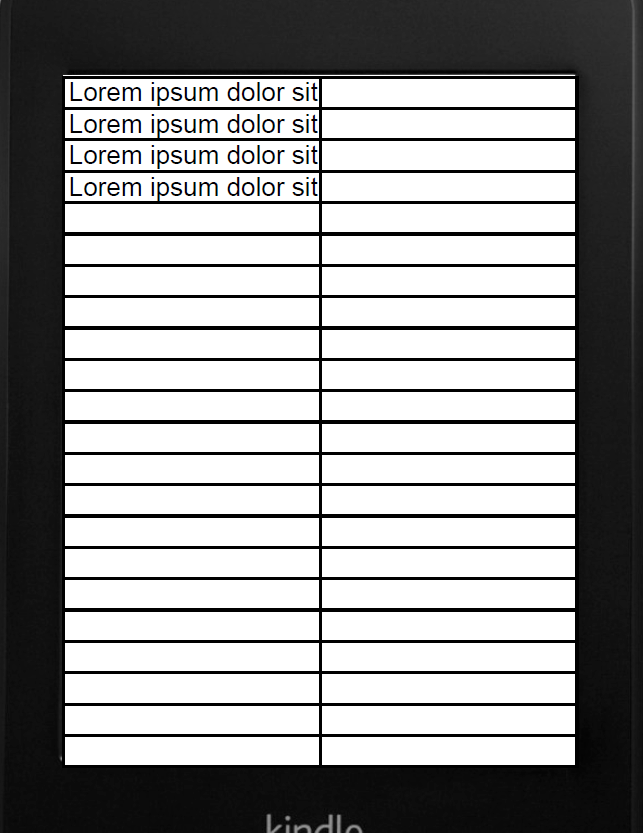
\includegraphics[width=0.3\textwidth]{gfx/float2.png}}\hspace{0.04\textwidth}
    \subfloat[][A 2-column float is encountered, and is inserted below the text]{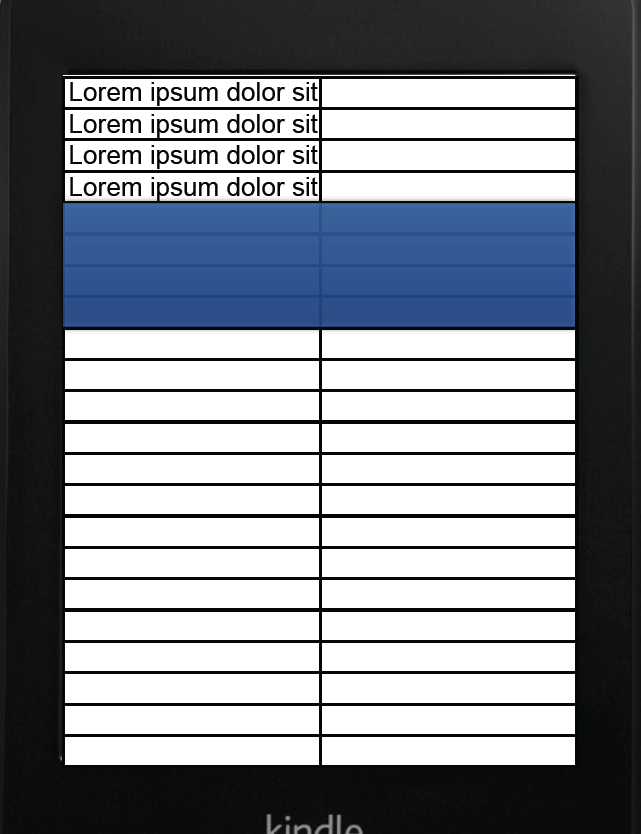
\includegraphics[width=0.3\textwidth]{gfx/float3.png}}\hspace{0.04\textwidth}
    \subfloat[][More lines of text are laid out]{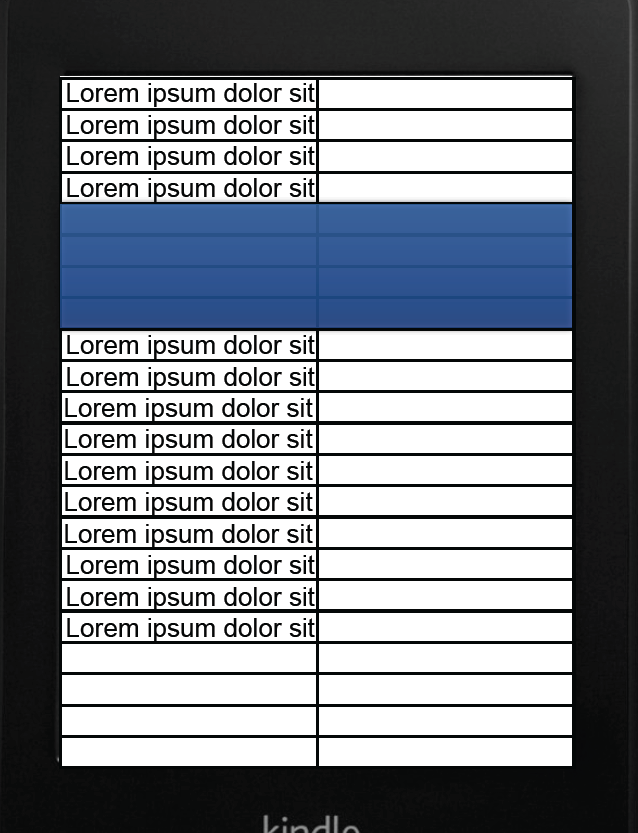
\includegraphics[width=0.3\textwidth]{gfx/float4.png}}\\
    \subfloat[][A single column float is encountered, but will not fit in the current space]{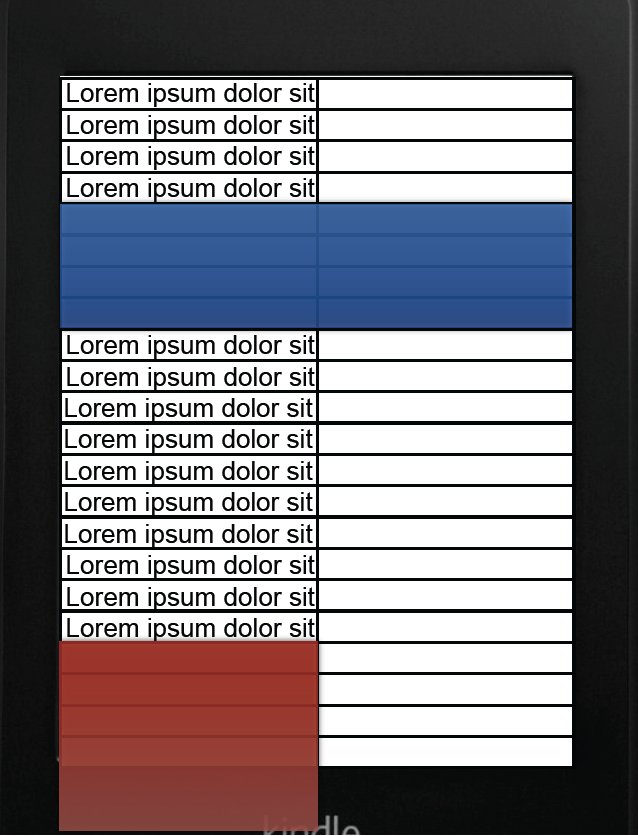
\includegraphics[width=0.3\textwidth]{gfx/float5.png}}\hspace{0.04\textwidth}
    \subfloat[][The float will also not fit at the top of the next column due to the position of the previous float]{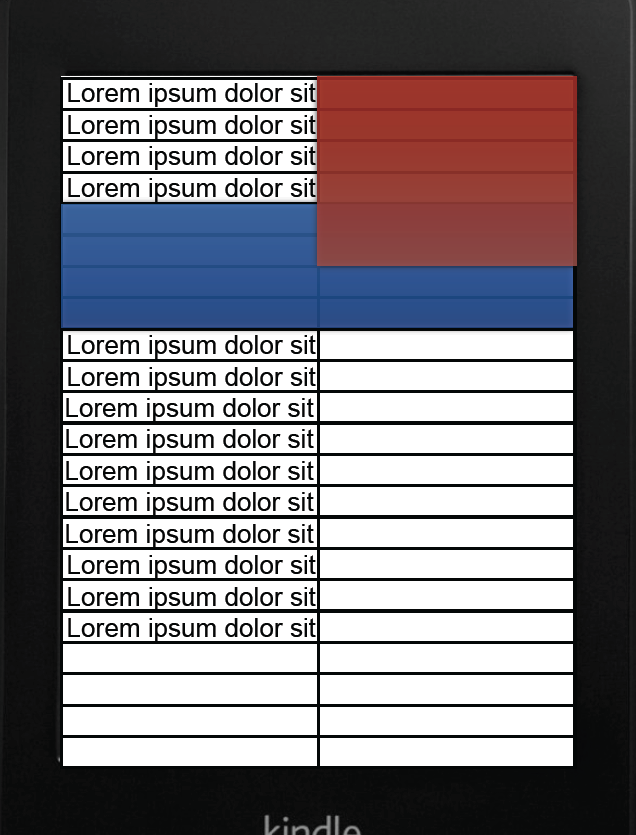
\includegraphics[width=0.3\textwidth]{gfx/float6.png}}\hspace{0.04\textwidth}
    \subfloat[][A space has been found for the second float]{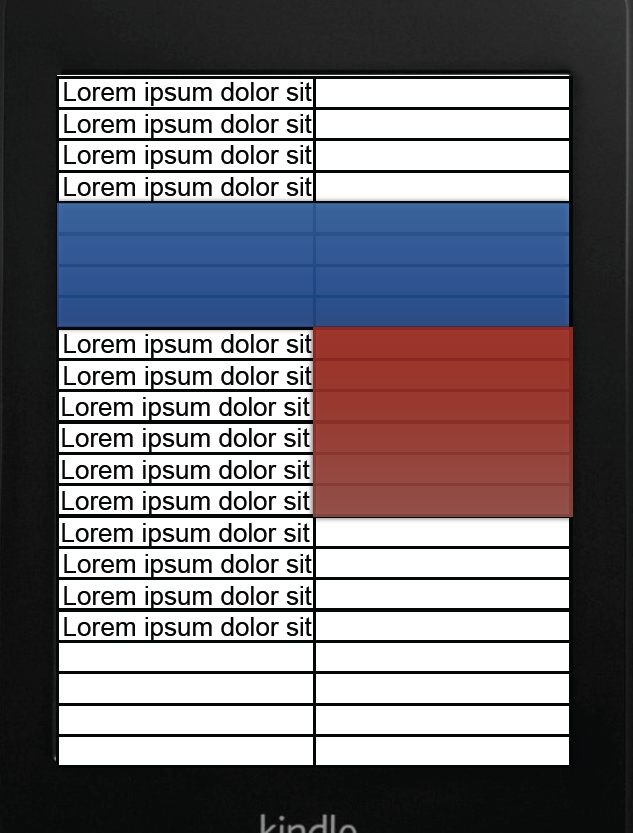
\includegraphics[width=0.3\textwidth]{gfx/float7.png}}\\
    \subfloat[][More text is laid out until the bottom of the column is reached]{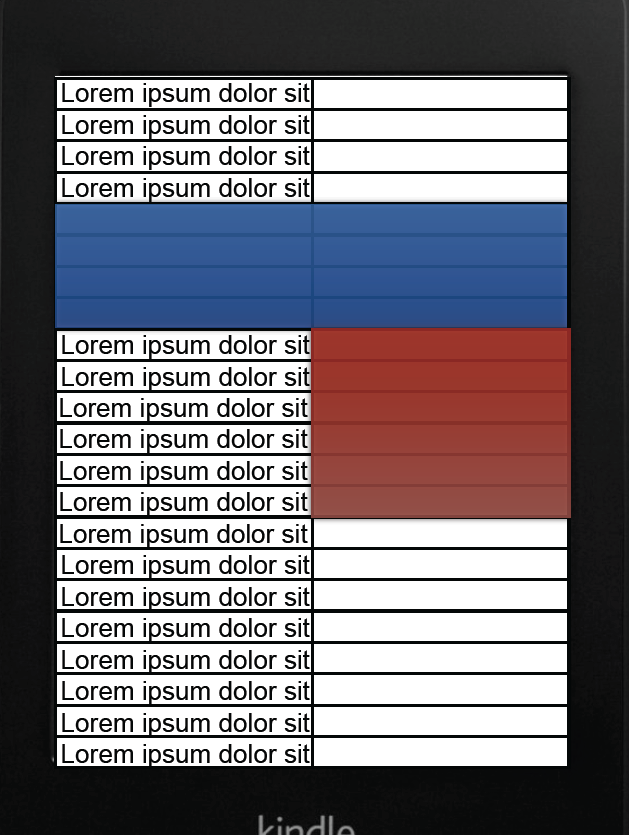
\includegraphics[width=0.3\textwidth]{gfx/float8.png}}\hspace{0.04\textwidth}
    \subfloat[][Text begins to be laid out at the top of the next column, until the reserved space of the float is encountered]{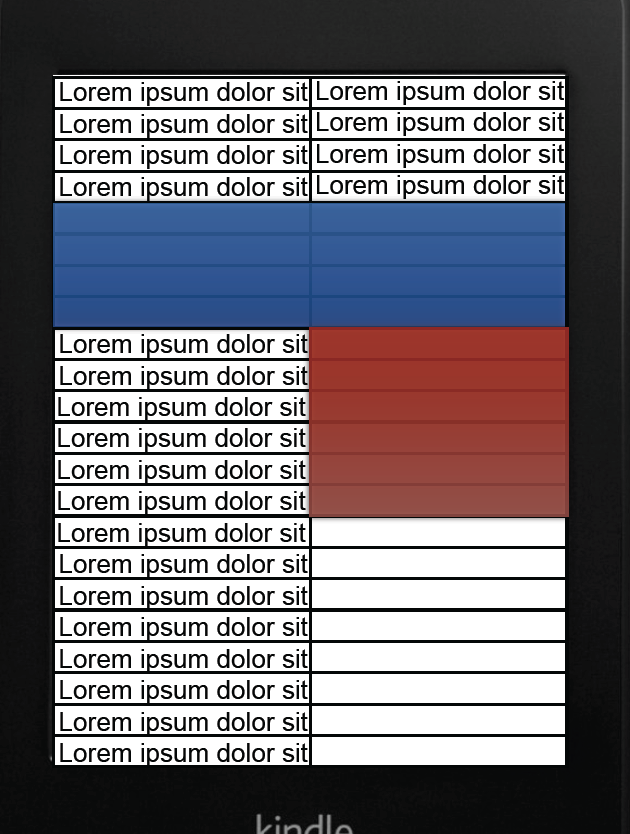
\includegraphics[width=0.3\textwidth]{gfx/float9.png}}\hspace{0.04\textwidth}
    \subfloat[][Text is subsequently laid out below the two floats until the page is filled]{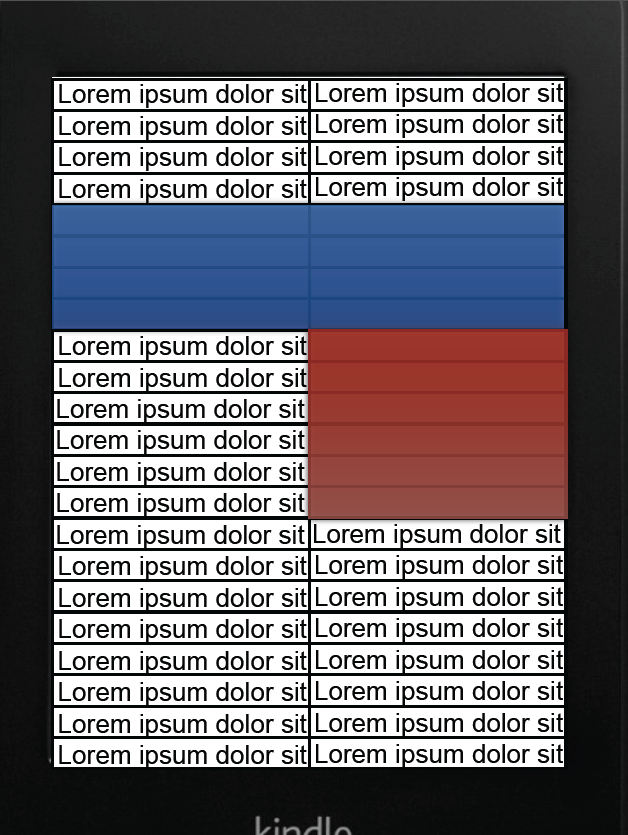
\includegraphics[width=0.3\textwidth]{gfx/float10.png}}
    \caption[Step through of multi-column layout]{A step-by-step example of how multi-column spanning floats are positioned using the grid-based layout described in Section~\ref{sec:gridlayout}}
    \label{fig:floatlayout}
\end{figure}



\begin{figure}
    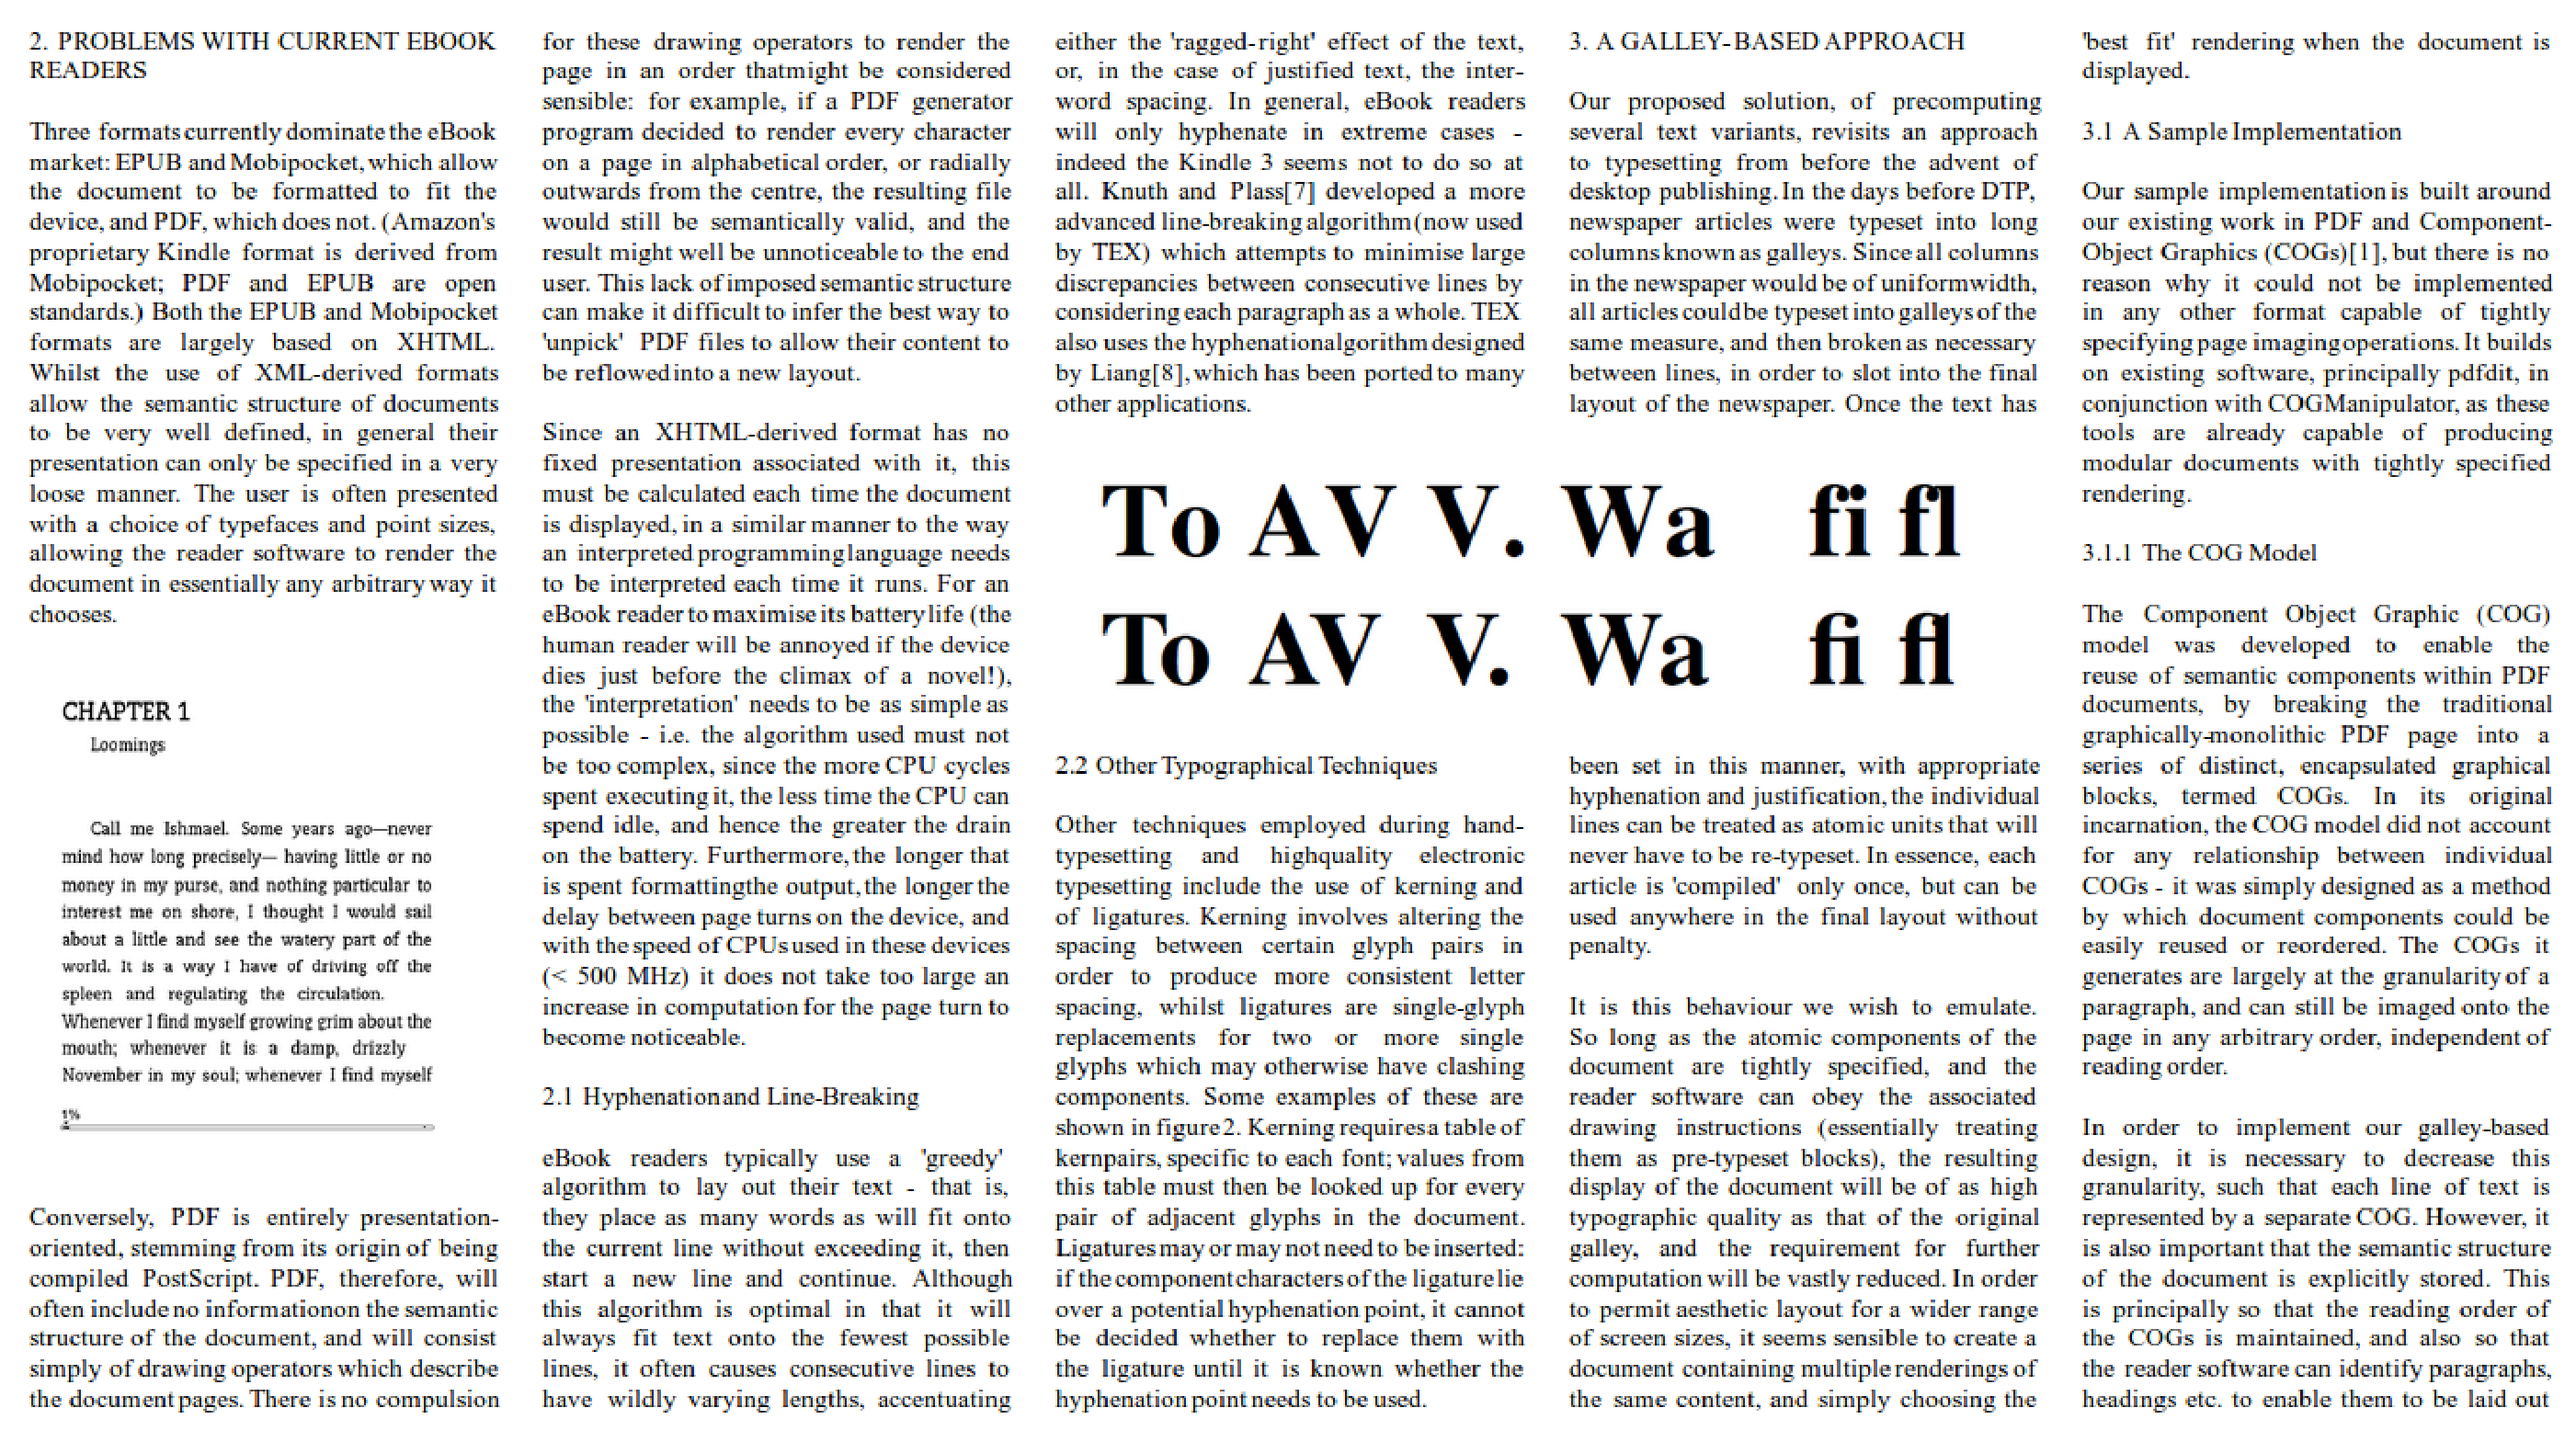
\includegraphics[angle=90,origin=c,width=\textwidth]{gfx/floatrendering}
    \caption[A sample rendering with multi-column floats]{An excerpt from \cite{Pinkney2011}, typeset and rendered by the system described in Chapter~\ref{ch:floats}. Of the two floats (a screenshot from a Kindle, and a demonstration of some micro-typographical techniques), one spans only one column, and one spans two. }
    \label{fig:screengrab}
\end{figure}


Pagination becomes a little trickier when floats are allowed to span multiple columns. For example, if a float whose natural size would lead it to span $n$ columns is encountered in the Galley Structure Tree when there are fewer than $n$ columns remaining to be typeset on the page, it must be decided how best to handle the situation. Three obvious options present themselves: alter the float to span fewer columns; delay the placement of the float until the start of the next page; or backtrack and check whether there is room to move the float back one or more columns, by shunting non-floatable text lines forwards.

The first option is clearly not ideal behaviour, given that shrinking a float may well reduce its legibility. Additionally, if this becomes a common problem, it is likely to be noticeable that floats spanning into the rightmost column of the page appear shrunken.

The second option (delaying placement until the following page) is a reasonable compromise, though it will increase float-drift (whereby floats become separated from their callout points in the text), which again is not ideal.

The third option (backtracking and shunting) is likely to produce the most desirable output, although some computational overhead will be added. One approach is simply to check whether there is enough space immediately to the left (specifically a gap between other, already placed, floats) into which the current float can be placed, with the displaced lines of text being shunted forwards. This method will not produce layouts as optimal as methods that use full backtracking and check all possibilities, but will run in much quicker time. A combination of all three of the above options is likely to work best in practice.


% \todo{Actually implement some of these pagination schemes, and write something intelligent-sounding about it. Provide some example output (screenshots).}

\section{Summary}

The reimplementation of the system in \html{} is not without its pitfalls. One strong advantage of using \pdf{} over \html{} is that any \pdf{} renderer that correctly implements the standard\hspace{0pt}\cite{ASI2001} should display any given document in an identical manner to any other renderer. Regrettably (and much to the chagrin of web developers everywhere) this is very much not true of rival web browser layout engines. Though standards do exist, published by the \gls{w3c},\footnote{See \url{http://www.w3.org/standards/} for full details} which are largely adhered to by all the major layout engines, there are certain areas that appear to be open to interpretation. One particular problem that is encountered, when using the system described in this chapter, is that of font scaling. 

The layouts produced by this system will only retain their quality if they are laid out precisely as specified by the typesetting process. Viewing the malleable documents in Google Chrome and Mozilla Firefox (which use WebKit and Gecko respectively) produces noticeably different results when the user chooses to scale the page up or down. WebKit appears to be inconsistent and non-linear when scaling fonts, whereas Gecko does a better job, and manages to lay out the text as intended by the typesetter. Figure~\ref{fig:craprenderer} shows an example of WebKit's font scaling problem. There is no real way around this issue, other than ensuring that whichever rendering engine is used in the reader device provides the required smooth scaling of fonts.

\begin{figure}
    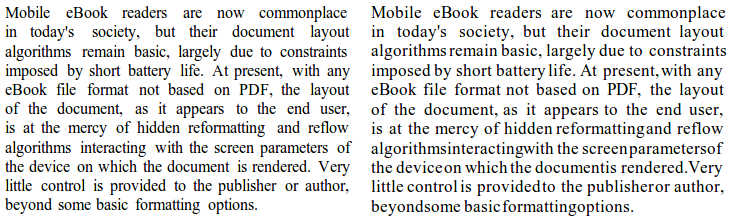
\includegraphics[width=\textwidth]{gfx/webkitisshit}
    \caption[Inconsistent font scaling by WebKit]{Chrome and Safari's layout engine (WebKit) can be inconsistent when scaling fonts. The paragraph to the left is displayed ``correctly'', but the paragraph to the right (scaled up by 1\% by the JavaScript) has clearly not scaled linearly. In contrast, Firefox's layout engine, Gecko, scales smoothly, and behaves as one might expect when zooming in on a \pdf{} file, which was the intended behaviour. (Output from Gecko is not shown in this figure.)}
    \label{fig:craprenderer}
\end{figure}

This is less of a problem on mobile devices: although in general their web browsers use the WebKit engine, their pixel-densities are much higher (many mobile phones have higher resolution screens than many laptops) so their displays are vastly scaled up, and fewer bad spacing issues such as those shown in Figure~\ref{fig:craprenderer} occur.

In general, however, as a document layout engine, the system produces professional-looking layouts that scale to fit on many different screen sizes, and the reimplementation in \textsc{xhtml}, \textsc{css}, and JavaScript makes the system much more portable. One stand-out problem remains: that of bloated filesizes. The next chapter proposes several methods to keep file sizes to a minimum.



%\todo{Write some analysis of the various float algorithms; provide some criticism of growing file sizes which leads onto the next chapter; mention problems that occur when the renderer tries to be clever (eg does its own kerning) ie Webkit vs Gecko}


